\chapter{Hardware modification enabling serial communication}
\label{appendix:uart_pins}

Here we describe the steps necessary to enable serial communication
between the watch and the PC. On the PC side serial port will be
emulated by the USB debug dongle. Figure \ref{fig:chronos_dongle_pins}
shows the functions of the dongle pins.
\begin{figure}[h]
  \centering
  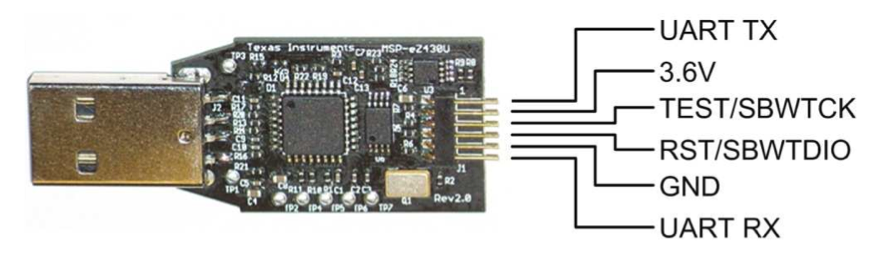
\includegraphics[width=0.7\textwidth]{img/chronos_dongle_pins.png}
  \caption{Pin functions of the USB debug dongle (Courtesy Texas Instruments)}
  \label{fig:chronos_dongle_pins}
\end{figure}
Ones labeled \emph{UART TX} and \emph{UART RX} are responsible for
serial communication. However if you look at chronos watch schematics,
you'll see that these pins remain unconnected in the watch. Relevant
snippet is shown in Figure \ref{fig:chronos_unonnected_uart}
\footnote{Schematics are published in \cite{eZ430Chronos}. For quick
reference, they were copied to the Appendix
\ref{appendix:watch_schematics}}.
\begin{figure}[h]
  \centering
  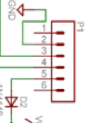
\includegraphics[width=0.14\textwidth]{img/chronos_unonnected_uart.png}
  \caption{Unconnected UART pins on the watch (Courtesy Texas Instruments)}
  \label{fig:chronos_unonnected_uart}
\end{figure}
This is exactly what needs to be changed. Fortunately the MCU is
capable of dynamic port remapping, which means that these UART pins may
be connected to any two IO pins and then the software can handle rest of the
configuration.

IO pins that are easiest to connect to the serial lines are those
responsible for watch buttons. The exact location of the connections
is presented in Figure \ref{fig:chronos_where_to_connect}.
\begin{figure}[h]
  \centering
  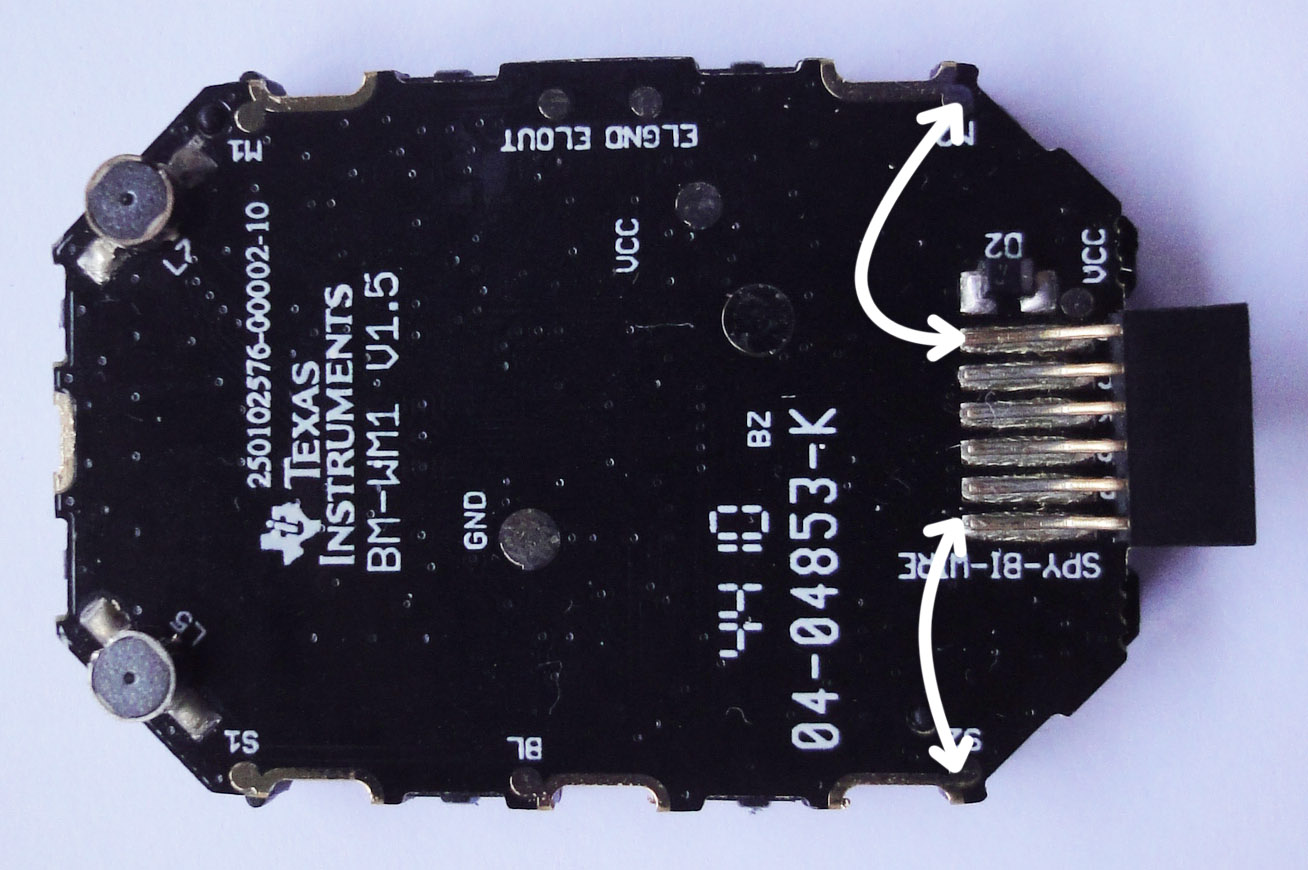
\includegraphics[width=0.7\textwidth]{img/chronos_where_to_connect.jpg}
  \caption{Location of new connections.}
  \label{fig:chronos_where_to_connect}
\end{figure}
Now we'll list steps necessary to perform the modification:
\begin{itemize}
  \item Take off the bottom circuit board cover. Loosen eight
    couplings, that hold it, with a small screwdriver as shown in
    Figure \ref{fig:chronos_cover_off}. Ensure you do not lose two
    tiny golden springs that connect power and buzzer to the board.
    \begin{figure}[h]
      \centering
      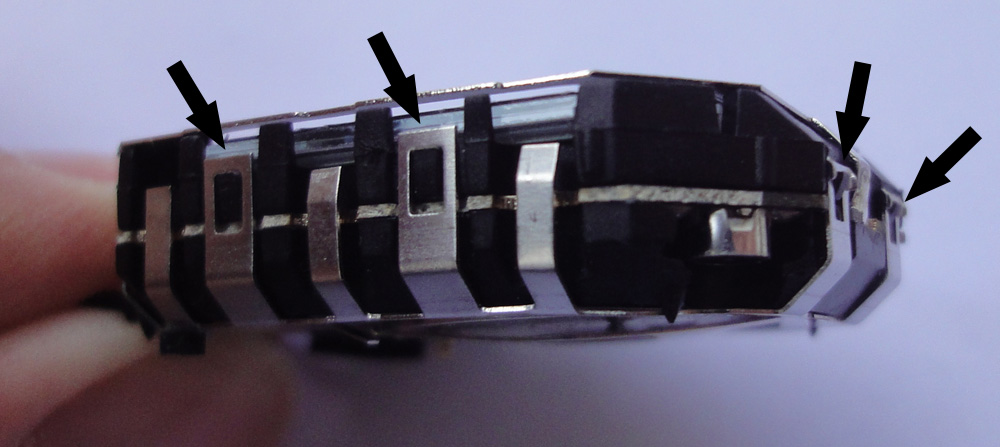
\includegraphics[width=0.8\textwidth]{img/chronos_cover_off.jpg}
      \caption{Couplings holding bottom circuit board cover.}
      \label{fig:chronos_cover_off}
    \end{figure}
  \item Take off the isolation of a piece of cooper wire. Cut two
    short pieces of it, that will make the connections.  Make sure
    their length is comfortable for soldering. Shape them until they
    form smooth paths between the connection points. Ensure that they
    will not contact to any other elements of the watch (SMT resistor
    near the connector).
  \item Place one of them in position and secure it with tape
    from one side.
  \item Solder the other side to the board. Bonding will now hold the
    wire in position. Remove the tape and solder the other end.
  \item Solder the second wire the same way. End result should
    look similarly to Figure \ref{fig:chronos_with_wires}.
    \begin{figure}[h]
      \centering
      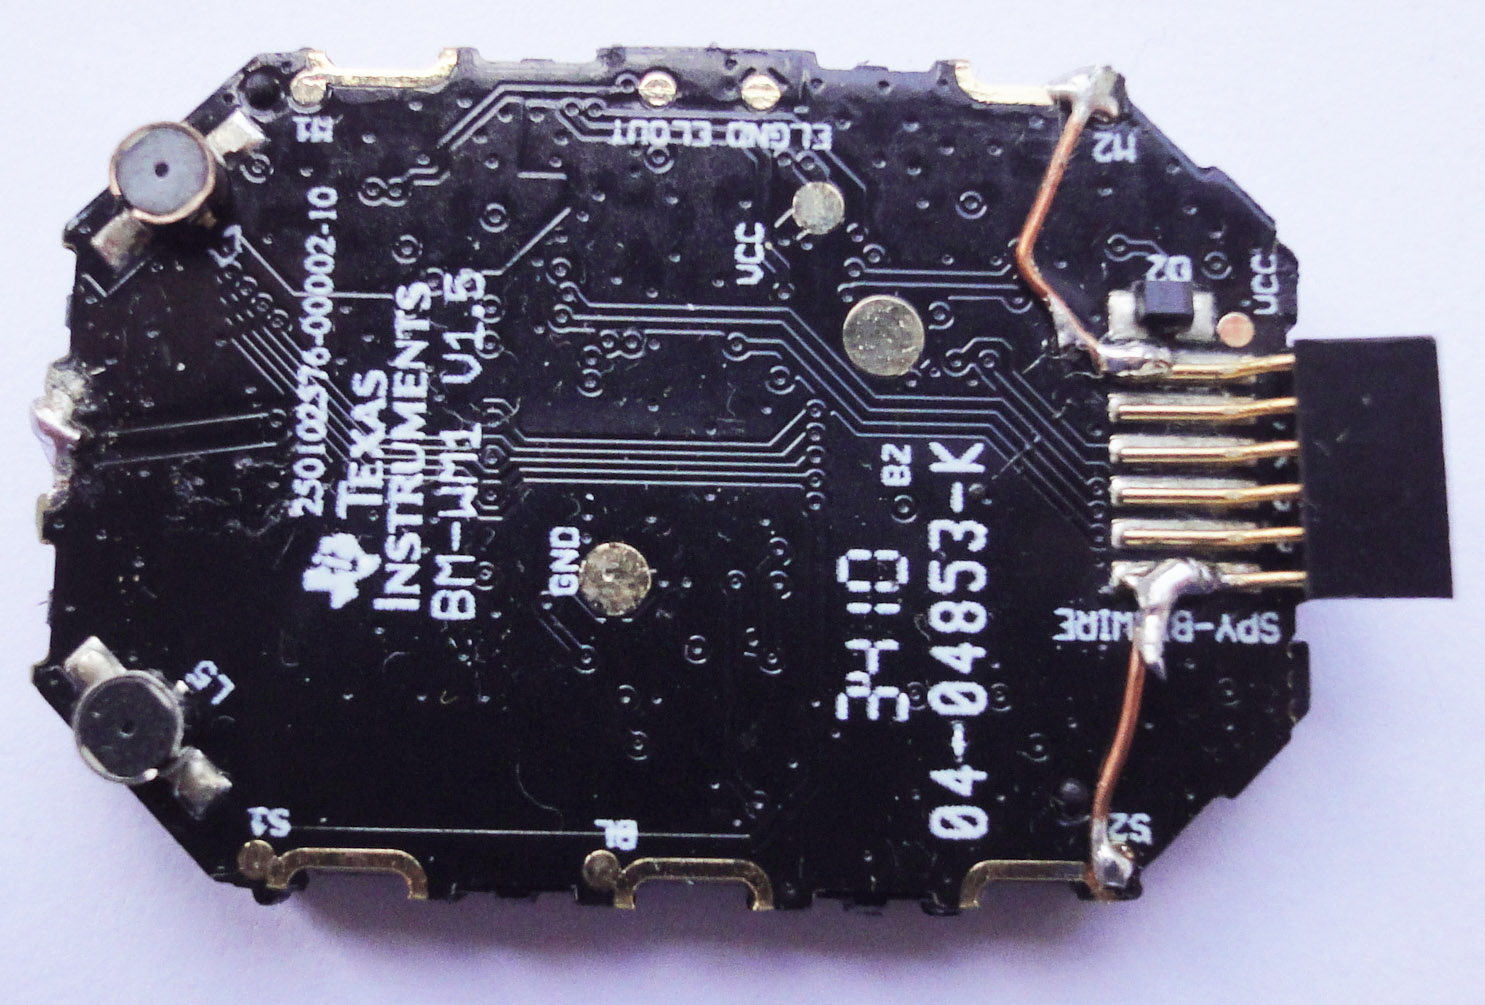
\includegraphics[width=0.6\textwidth]{img/chronos_with_wires.jpg}
      \caption{Watch's circuit board with UART connections.}
      \label{fig:chronos_with_wires}
    \end{figure}
  \item Put the cover back on. Ensure that two small golden springs
    are in position.
  \item Test the device, by running TinyOS TestSerial application. See
    it's \emph{README.txt} file for detailed instructions.  Note that
    certain unreliability of the serial port is to be expected.  1 :
    1500 error rate is well within tolerance.
\end{itemize}

%------------------------------------------------------------------------------

\chapter{Chronos watch schematic}
\label{appendix:watch_schematics}

\centering
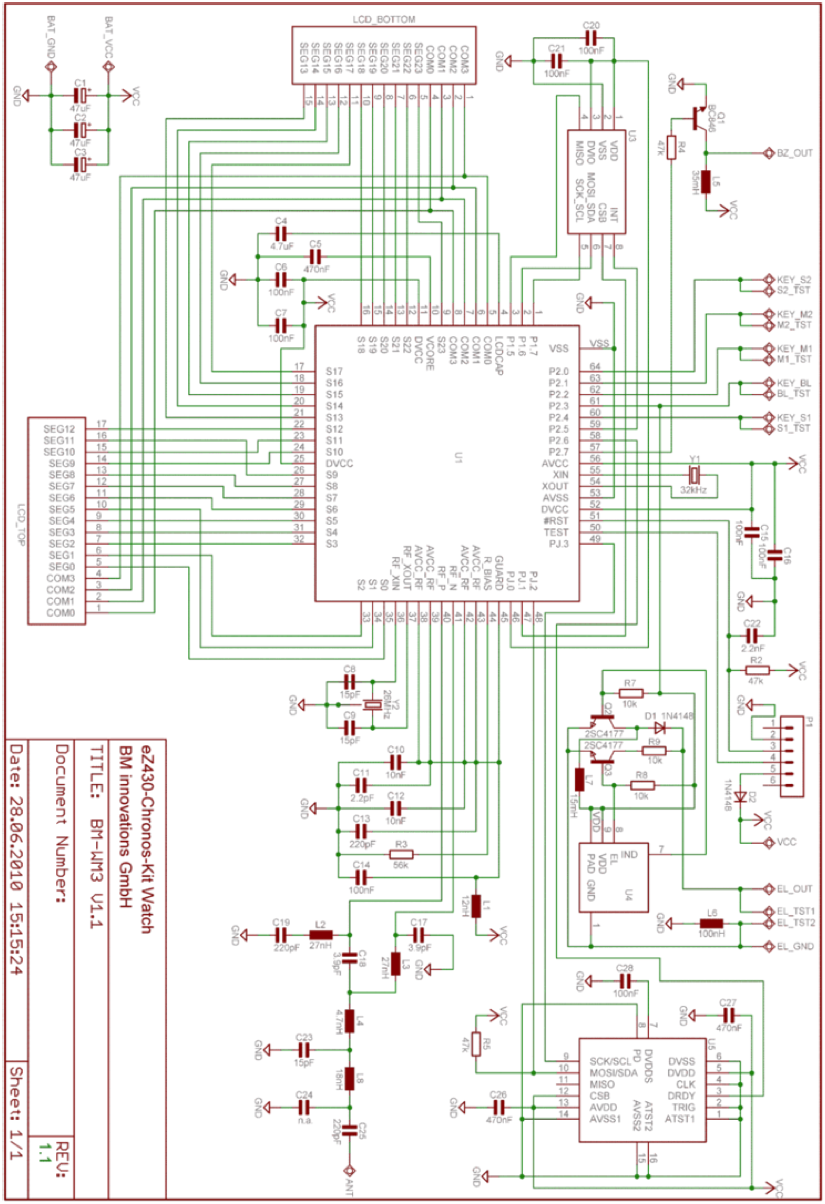
\includegraphics[width=0.75\textwidth]{img/watch_schematics.png}

%------------------------------------------------------------------------------
% Porzucone

% \chapter{Chronos development environment installation}
% \label{appendix:env_install}
% 
% In this appendix, we describe steps necessary to install compilers and
% other software necessary to develop software for Chronos platform.



% Vim settings:
% vim: set textwidth=70:
% vim: set fo+=t:
